\section{Componentes principales}
\setcounter{sectiontotal}{5}

\begin{frame}
    \frametitle{\pagetitle}
    \framesubtitle{Arquitectura}
    %\pause{}
	\begin{figure}
		%\centering
        \includegraphicsx[scale=0.41]{../tecnologias/images/full.pdf}
		\caption{Esquema general de componentes de la solución}
	\end{figure}
\end{frame}

\begin{frame}
\frametitle{\pagetitle}
\framesubtitle{Motor de videojuego: Unity 3D}
\tiny

\begin{tabulary}{\textwidth}{rCCCCCCCC}
\toprule
& \multicolumn{3}{c}{\textbf{Motor}\footnote{\fullcite{videojuego:telechea}}} \\

\cmidrule(lr){2-4}  
\textbf{Característica}         &
\textbf{Unreal Engine}          &
\textbf{CryEngine}              &
\textbf{Unity3D}                \\
\midrule
\textbf{Distribución} & iOs. Otros en la versión comercial. & iOs, Android & {\color{blue!90!black}
Android, Windows Phone, iOs, BlackBerry} \\ 

\midrule
\textbf{Tienda} & Mediana & Mediana & \color{blue!90!black} Grande \\

\textbf{Comunidad} & Grande & Mediana & {\color{blue!90!black} Grande} \\

\midrule
\textbf{Formatos} & fbx, dds, raw, ASE & Formatos propios & {\color{blue!90!black} FBX, OBJ,
Max, Blend, dae, 3ds, dxf, MB, MA, etc} \\

\midrule
\textbf{Curva de aprendizaje} & Compleja & Compleja & {\color{blue!90!black} Sencilla} \\

\textbf{Lenguajes} & Unreal Script y C++ & C++, Lua & {\color{blue!90!black} \cs{}, UnityScript y Boo} \\

\midrule
\textbf{Licencia del motor} & Versiones antiguas gratuitas para uso no comercial. &
Gratuita solo para uso no comercial & {\color{blue!90!black} Versión limitada
gratuita, disponible para uso no comercial} \\

\textbf{IDE} & Si, gratuito no comercial & Sí, propietario & {\color{blue!90!black} Sí,
gratuito no comercial} \\
\bottomrule

\end{tabulary}

\end{frame}



\begin{frame}
\frametitle{\pagetitle}
\framesubtitle{Arquitectura}
\begin{figure}
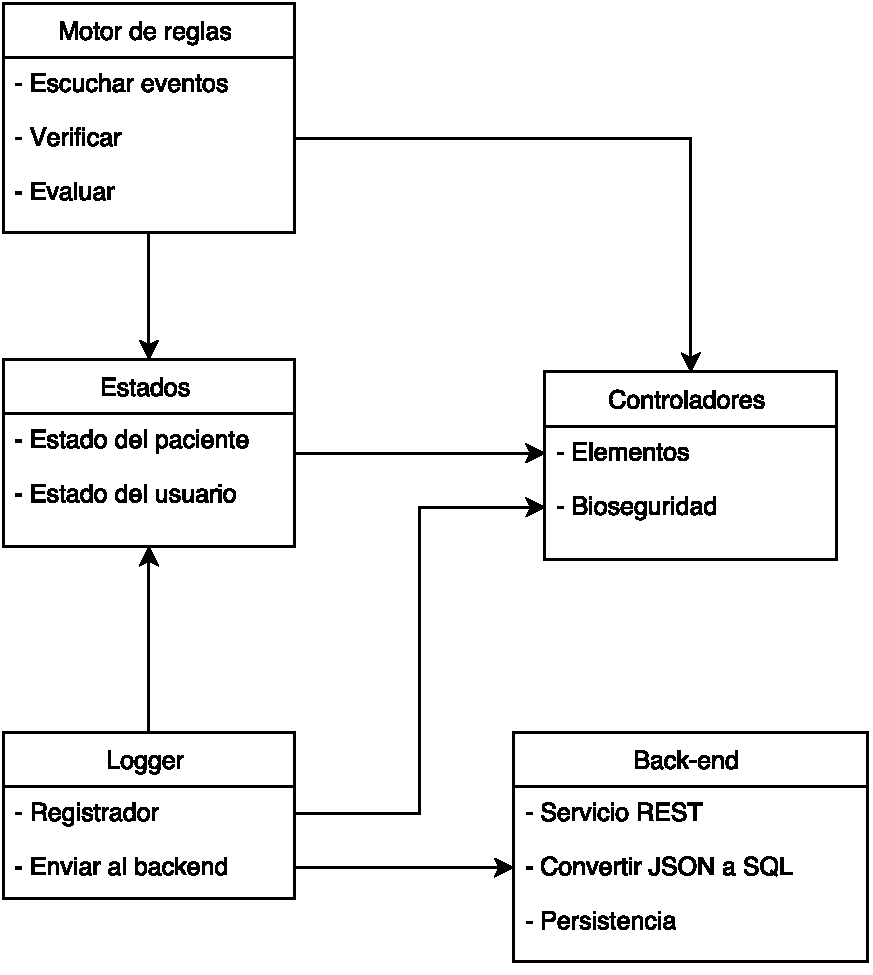
\includegraphics[width=\textwidth,height=0.7\textheight,keepaspectratio]{./imagenes/esquema_global.pdf}
\end{figure}
\end{frame}

\begin{frame}
\frametitle{\pagetitle}
\framesubtitle{Tecnologías utilizadas \- Front-end}
\begin{table}
\centering
\begin{tabular}{lrr}
\toprule
\textbf{Utilización} & \textbf{Tecnología} \\
\midrule
Motor de videojuego      & Unity3d         \\
IDE                      & MonoDevelop     \\
                         & Unity Editor    \\
\midrule
Modelado 3D              & 3ds Max         \\
Modelado 2D              & Photoshop       \\
Modelado de personajes   & MakeHuman       \\

\midrule
Lenguaje de programación & \cs{} \\
Gestión de código fuente & Git \\
Otras librerías          & NGUI            \\
                         & Facebook \\
                         
\bottomrule
\end{tabular}
\end{table}
\end{frame}

\begin{frame}
\frametitle{\pagetitle}
\framesubtitle{Tecnologías utilizadas \- Back-end}
\begin{table}
\centering
\begin{tabular}{lrr}
\toprule
\textbf{Utilización} & \textbf{Tecnología}  \\
\midrule
IDE                         & Eclipse \\
Lenguaje de programación    & Java \\
\midrule
Servidor de aplicaciones    & Jboss \\
Servidor de base de datos   & PostgreSQL \\
Proveedor de plataforma     & OpenShift \\
\midrule
Gestión de código fuente    & Git & 1.8\\
Otras librerias             & Java EE & 6\\

\bottomrule
\end{tabular}
\end{table}
\end{frame}
